
%----------------------------------------------------------------------------------------
%	PACKAGES AND THEMES
%----------------------------------------------------------------------------------------

\documentclass[aspectratio=169]{beamer}
\mode<presentation> {
	
	\usetheme{Boadilla}
}
\definecolor{lmugreen}{RGB}{0, 136, 58}
\usecolortheme[named=lmugreen]{structure}
\usepackage{graphicx} % Allows including images
\usepackage{booktabs} % Allows the use of \toprule, \midrule and \bottomrule in tables
\usepackage[english]{babel}
\usepackage[utf8]{inputenc}
\usepackage{amsmath,amssymb} % math symbols
\usepackage{graphicx}
\usepackage{float}
\usepackage{tikz} % for DAGs
\usetikzlibrary{arrows.meta, positioning}
\usepackage{hyperref} % for URLs
\newcommand{\gray}{\rowcolor[gray]{.90}}
\usepackage{verbatim}
\usepackage{textpos} % logo position
\usepackage[default]{sourcesanspro} % font type
\usepackage{cases} % math cases

% Caption
\usepackage{caption}
\DeclareCaptionFont{tiny}{\tiny}
\captionsetup{font=scriptsize,labelfont=scriptsize,justification=centering}

% ToC
\AtBeginSection[]{
	\begin{frame}[noframenumbering, plain]
	\frametitle{Outline}
	\setcounter{tocdepth}{1}
	\tableofcontents[currentsection]
\end{frame}
}

% Remove navigation 
\beamertemplatenavigationsymbolsempty

% R 
\usepackage{listings}
\lstset{
language=R,
basicstyle=\scriptsize\ttfamily,
commentstyle=\ttfamily\color{gray},
backgroundcolor=\color{white},
showspaces=false,
showstringspaces=false,
showtabs=false,
tabsize=2,
captionpos=b,
breaklines=false,
breakatwhitespace=false,
title=\lstname,
escapeinside={},
keywordstyle={},
morekeywords={}, 
belowskip = -1.2 \baselineskip,
}

%----------------------------------------------------------------------------------------
%	TITLE PAGE
%----------------------------------------------------------------------------------------

\addtobeamertemplate{frametitle}{}{%
	\begin{textblock*}{100mm}(0.88\textwidth,-0.5cm)
		
\includegraphics[height=1cm,width=2cm]{../figures/lmu_logo}
\end{textblock*}}

%
\includegraphics[width=0.3\textwidth]{lmu_logo}
\vspace*{-1cm}

\title{Your Title} 

\author{Your Name} 
\institute[LMU]{LMU} % Your institution as it will appear on the bottom of every slide, may be shorthand to save space
{

}
\begin{document}

{
\usebackgroundtemplate{
\includegraphics[width=\paperwidth]{../figures/lmu-background.pdf}}
\begin{frame}
\begin{columns}
	\begin{column}{0.4\textwidth}
		\vspace{3cm}
		
		\textbf{\textcolor{white}{\Large Your Title}}
		\vspace{1cm}
		
		\textcolor{white}{\footnotesize Your Name \\
			\today}
	\end{column}
	\begin{column}{0.49\textwidth}
		\vspace{2cm}
		\begin{center}
			
\includegraphics[width=1\textwidth]{../figures/showcase_figure.png}
		\end{center}
	\end{column}
\end{columns}
\end{frame}
}
%----------------------------------------------------------------------------------------
%	PRESENTATION SLIDES
%----------------------------------------------------------------------------------------

\section{Daten und Kontext}
\section{Fairness Definitionen}
\section{Quellen von Bias}
\section{Methoden für Fairness}

\begin{frame}{Daten und Kontext}
	\begin{itemize}
		\item "begründeter Verdacht" ("reasonable suspicion") als Grund für Polizeikontrolle
		\item "wahrscheinliche Ursache" ("probable cause") als Grund für Festnahme
		\item Mögliche Resultate:
		\begin{itemize}
			\item Keine weiteren Maßnahmen
			\item Schnelle Abtastung (frisk)
			\item Durchsuchung (search)
			\item Festnahme (arrest)
		\end{itemize}
		\item Kritik, dass Strategie diskriminierend gegenüber Schwarzen und Latinos ist
		\item Modellieren des Entscheidungsprozesses für Festnahme mit RF
		\item \texttt{race} als protected attribute (PA)
	\end{itemize}
\end{frame}
	
\begin{frame}
    \frametitle{Fairness Definitionen}
    \begin{itemize}
        \item Fairness Definitionen
        \begin{itemize}
            \item Gruppen Fairness/ Statistische Fairness
            \item Individuelle Fairness
            \item Kausale Fairness
        \end{itemize}
    \end{itemize}
    
    % Add annotations and arrows using TikZ
    \begin{tikzpicture}[overlay, remember picture]
        % Position for the "Entscheidung -|-> Ungleichheit" annotation
        \node[align=left, anchor=west] at (10, 1) (stat-comment) {Entscheidung \\ $-\!\!\!-\!\!\!| \to$ \\ Ungleichheit};
        
        % Position for the "Merkmale -|-> Entscheidung" annotation
        \node[align=left, anchor=west] at (5.5, -1) (relation-comment) {Merkmale \\ $-\!\!\!-\!\!\!| \to$ \\ Entscheidung};
        
        % Arrow from Gruppen Fairness to "Entscheidung -|-> Ungleichheit"
        \draw[-{Latex}, thick] (2, 1.2) -- (stat-comment.west);
        
        % Arrow from Individuelle and Kausale Fairness to "Merkmale -|-> Entscheidung"
        \draw[-{Latex}, thick] (2, 0) -- (relation-comment.west);
        \draw[-{Latex}, thick] (2, -0.5) -- (relation-comment.west);
    \end{tikzpicture}
\end{frame}



\begin{frame}
	\frametitle{Gruppen Fairness}
	Idee: Gruppen von Personen erfahren Diskriminierung aufgrund dieser Gruppenzugehörigkeit
	Unterkategorien:
	\begin{itemize}
		\item Unabhängigkeit: $\hat{Y} \perp A$
		\item Separierbarkeit: $\hat{Y} \perp A | Y$ 
		\item Suffizienz: $Y \perp A | \hat{Y}$
	\end{itemize}
\end{frame}

\begin{frame}
	\frametitle{Unabhängigkeit}
	Statistical Parity
	$$P(\hat{Y} = 1 | A = a) = P(\hat{Y} = 1 | A = b)$$
\end{frame}

\begin{frame}
	\frametitle{Separierbarkeit}
	Fokus liegt auf gleichen Fehlerraten
	Herleitung anhand der Fehlermatrix
	\begin{table}[H]
	\centering
	\begin{tabular}{c|c|c}
	\toprule
	 & $\hat{Y} = 1$ & $\hat{Y} = 0$ \\
	\midrule
	$Y = 1$ & True Positive (TP) & False Negative (FN) \\
	$Y = 0$ & False Positive (FP) & True Negative (TN) \\
	\bottomrule
	\end{tabular}
	\caption{Error Matrix}
	\end{table}
	% DAG for Separation
	\begin{figure}[H]
	\centering
	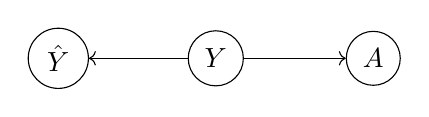
\begin{tikzpicture}
		\node[draw, circle] (Y) at (0,0) {$Y$};
		\node[draw, circle] (A) at (2,0) {$A$};
		\node[draw, circle] (Yhat) at (-2,0) {$\hat{Y}$};
		\draw[->] (Y) -- (A);
		\draw[->] (Y) -- (Yhat);
	\end{tikzpicture}
	\caption{Simple Graphical Model}
	\end{figure}
	$$P(\hat{Y} = 1 | A = a, Y = y) = P(\hat{Y} = 1 | A = b, Y = y)$$
\end{frame}

\begin{frame}
	\frametitle{Suffizienz}
	Positive/negative Vorhersage soll die selbe Bedeutung für alle Gruppen haben
	$$P(Y = 1 | A = a, \hat{Y} = \hat{y}) = P(Y = 1 | A = b, \hat{Y} = \hat{y})$$
	Erweiterung davon bedingt auf den Score, nicht das Label: Calibration
\end{frame}
\begin{frame}
	\frametitle{Advantages and Disadvantages}
	\begin{table}[H]
	\centering
	\begin{tabular}{c|c}
	\toprule
	$+$ & $-$ \\
	\midrule
	Leicht verständlich & Infragmarginality \\
	Leicht einzubauen in existierende Optimierungskriterien & Observational \\
	\bottomrule
	\end{tabular}
	\caption{Advantages and Disadvantages}
	\end{table}
	--> Scheint erstmals sinvoller und simpler Ansatz zu sein. Schaut man etwas tiefer stellt sich
	die Fragem ob die Metriken wirklich geeignet sind um Fairness zu erhöhen
	Aktuelle Literatur weist darauf hin, dass sie eher Ausdruck der Zufallsverteilung
	von $\hat{Y}, Y, A, X$ sind
\end{frame}

\begin{frame}
    \frametitle{Individuelle Fairness}
    \begin{enumerate}
        \item Fairness through Unawareness (FTU) = Blinding
        \begin{itemize}
            \item Vorgehensvorschrift: PA soll nicht im Entscheidungsprozess verwendet werden
            \item Keine eindeutige mathematische Definition, sondern verschiedene Ansätze zum Testen von FTU
            \item Erweiterung: PA und alle Proxies dürfen nicht im Entscheidungsprozess verwendet werden
        \end{itemize}
        
        \item Fairness through Awareness (FTA)
        \begin{itemize}
            \item Ähnlichkeit im Feature Space soll zu Ähnlichkeit im Prediction Space führen
            \item Lipschitz-Kriterium:
            \[
            d(\hat{y_i}, \hat{y_j}) \leq \lambda d(x_i, x_j)
            \]
            \item Lässt sich in ein lineares Optimierungsproblem umformulieren
            \item Definition des Distanzmaßes $d$ im Feature Space ist eine Herausforderung
        \end{itemize}
    \end{enumerate}
\end{frame}


\begin{frame}
	\frametitle{Kausale Fairness}
	Ziel ist hier die kausalen Struktur der Daten zu verstehen
	Fairness als pipeline Problem (Fairness + ML)
	\begin{itemize}
		\item Counterfactual Fairness
		\item Definition über DAGs
	\end{itemize}
\end{frame}

\begin{frame}
	\frametitle{Fairness Methoden}
	\begin{itemize}
		\item Preprocessing
		Daten vor dem Training bearbeiten
		\item Inprocessing
		Trainingsprozess anpassen, Optimierungsproblem modifizieren
		\item Postprocessing
		Vorhersagen nach dem Training bearbeiten
	\end{itemize}
\end{frame}


\end{document}


